
\section{Background}

In this section, we provide a brief introduction to contact modeling with the
linear complementarity formulation.
%
We also present a summary of the mixture of experts architecture and
its uses in machine learning.

\subsection{Contact Modeling with Linear Complementarity Problem}

Suppose a hybrid dynamical system consists of $k$ contact events, each
introducing normal contact forces $\lambda_N \in \mathbb{R}^{k}$ and Coulomb
friction forces $\lambda_T \in \mathbb{R}^{k}$ to the overall system.
%
We can model this hybrid system with the measure equality~\cite{glocker2005formulation}

\begin{equation}
  \begin{gathered}
    M(q) \dd \dot{q} + h(q, \dot{q})\dd t - \dd R  = 0, \\
    h(q, \dot{q}) = C(q, \dot{q})\dot{q} + G(q) - Bu(q, \dot{q}), 
  \end{gathered}
  \label{eq:hybrid_dynamics}
\end{equation}

\noindent where $x \in \mathcal{X} \subset \mathbb{R}^{2m}$ consists of robot
position $q \in \mathbb{R}^m$ and velocities $\dot{q}$, $M \in \mathbb{R}^{m
\times m}$ denotes the positive-definite mass matrix, $C \in \mathbb{R}^{m
\times m}$ holds the Coriolis and centripetal terms, and $G \in \mathbb{R}^{m}$
is the gravitational term. The matrix $B \in \mathbb{R}^{m \times n}$ maps the
input $u \in \mathbb{R}^{n}$ to the generalized coordinates and $\dd R \in
\mathbb{R}^m$ represents the force measure of contact forces and Coulomb
friction exerted on the system. 
%
% The vector $\lambda \in \mathbb{R}^{2k}$ consists of the normal and
% tangential contact forces and the matrix $W \in \mathbb{R}^{m \times 2k}$ maps
% these contact forces to the generalized coordinates.
%
In contrast to smooth dynamical systems, the hybrid
system~\eqref{eq:hybrid_dynamics} exhibits contact forces that enforce
the geometric and kinematic constraints of surfaces in contact.
%
For instance, the contact force between two objects in collision characterizes
the no-penetration conditions and the post-impact velocities of the objects.
%
Resolving these contact forces accurately can be difficult and computationally
expensive.
%
Most collision simulators work on the kinematic level as opposed to the dynamic
level.
%
For instance, there are event detection methods that simply change the velocity
of the moving objects at the time of impact.
%
One of the drawbacks of these techniques is finding the exact time the contact
occurs in high speed collision.
%
There is the additional difficulty of identifying the Coulomb friction, which is
especially prone to Painlev{{\'e}} Paradox~\cite{genot1999new} in high friction
scenarios.
%
The linear complementarity formulation in~\cite{glocker2005formulation} provides
a rigorous technique to resolve contact forces, Coulomb friction and impact
forces in a hybrid system.
%
The work presents an optimization problem that searches for \it{contact force
and post-impact velocity} \normalfont pairs that obey the geometric and
kinematic constraints during contacts or impacts.
%

%
The linear complementarity formulation is constructed as follows. We define a
vector of gap functions $g_N(q) \in \mathbb{R}^{k}$ that measure the
Euclidean distance between the contact surfaces. 
%
Let $\gamma_N = \dot{g}_N(q)$ be the normal relative velocity and
$\gamma_T$ the tangential relative velocity between contact surfaces.
%
The linear complementarity formulation imposes a unilateral constraint between
contact forces and relative velocities given by:

\begin{equation}
  \begin{gathered}
    0 \leq 
    \begin{pmatrix}
      \xi_N(q, \dot{q}) \\
      \xi_T(q, \dot{q})
    \end{pmatrix} 
    \perp
      \begin{pmatrix}
        \lambda_N  \\
        \lambda_T
      \end{pmatrix} \geq 0, \\
  % \end{eqnarray}
  % \begin{eqnarray}
    \begin{pmatrix}
      \xi_N(q, \dot{q}) \\
      \xi_T(q, \dot{q})
    \end{pmatrix} =
      \begin{pmatrix}
        (1+\epsilon_N) \gamma_N(q, \dot{q})  \\
        (1+\epsilon_T) \gamma_T(q, \dot{q})
      \end{pmatrix},
  \end{gathered}
  \label{eq:complementarity} 
\end{equation}

\noindent where $\epsilon_N$ and $\epsilon_T$ are the normal and tangential
coefficients of restitution respectively. 
% 
From the dynamics in~\eqref{eq:hybrid_dynamics}, $\xi_N$ and $\xi_T$ can be
expressed as an affine function over the contact forces $\lambda_N$ and
$\lambda_T$ as follows~\cite{glocker2005formulation}:

\begin{gather*}
  \begin{pmatrix}
    \xi_N \\
    \xi_R \\
    \lambda_L
  \end{pmatrix} =
      A
    \begin{pmatrix}
      \lambda_N \\
      \lambda_R \\
      \xi_L
    \end{pmatrix} + b, \\
    A = \begin{bmatrix}
      W_N M^{-1} (W_N - W_T \mu) & W_N M^{-1} W_N & 0  \\
      W_T M^{-1} (W_N - W_T \mu) & W_T M^{-1} W_T & I_k  \\
      2\mu & -I_k & 0
    \end{bmatrix}, \;  b = \begin{bmatrix}
      W_N M^{-1} h \Delta t + (I_k+\epsilon_N) \gamma_N\\
      W_T M^{-1} h \Delta t + (I_k+\epsilon_T) \gamma_T\\
      0
    \end{bmatrix} \\
    \begin{pmatrix}
      \xi_T   \\
      \lambda_R \\
      \lambda_L 
    \end{pmatrix} = 
    \begin{pmatrix}
      \xi_R - \xi_L \\
      \mu \lambda_N + \lambda_T  \\
      \mu \lambda_N - \lambda_T  
    \end{pmatrix} \\
\end{gather*}
 
\noindent where $\mu$ is the coefficient of friction, $I_k$ is the $k \times k$ identity
matrix, $W_N$ and $W_T$ map the velocity vector $\dot{q}$ to $\gamma_N$ and
$\gamma_T$, respectively, and $\Delta t$ is the integration time step.
%
The linear complementarity problem (LCP)~\eqref{eq:complementarity} can be posed as
the following feasibility problem:

\begin{equation}
    0 \leq 
    \left[ A \begin{pmatrix}
      \lambda_N \\
      \lambda_R \\
      \xi_L
    \end{pmatrix} + b \right]
    \perp
    \begin{pmatrix}
      \lambda_N \\
      \lambda_R \\
      \xi_L
    \end{pmatrix} \geq 0, \\
  \label{eq:feasibility} 
\end{equation}
\noindent which can be solved with various optimization techniques. 

We follow Moreau's time stepping algorithm~\cite{glocker2005formulation}
outlined in Algorithm~\eqref{algo:moreau} to resolve the complementarity
constraint in~\eqref{eq:feasibility} and numerically integrate the
dynamics~\eqref{eq:hybrid_dynamics}. While the complementarity constraint can be
posed as a feasibility problem, the presence of Coulomb friction makes it a
non-convex optimization problem. We use a pivoting (basis-exchange) technique
called Lemke's algorithm~\cite{acary2008numerical} to find the solution to the
linear complementarity problem~\eqref{eq:feasibility}. This allows us to
differentiate the solution to the LCP in our efforts to use machine learning
techniques.

\begin{algorithm}[H]
  \setstretch{1.2}
    \caption{Moreau's Time Stepping Algorithm}
    \label{algo:moreau}
    \small
    \hspace*{\algorithmicindent} \textbf{Input}: $x(0) = (q(0), \dot{q}(0))$
    \begin{algorithmic}[1]
      \State $\phi \leftarrow  [x(0)]$ \Comment{Initial States}
        % \algrenewcommand\algorithmicindent{0em} % No indent
          \For{$t = 0:\Delta t:T$} \Comment{Time stepping}
            \State $t_M = t + \nicefrac{\Delta t}{2}$
            \State $q(t_M) = q(t) +  (\nicefrac{\Delta t}{2}) \dot{q}(t) $\Comment{Half-time step integration}
            % \State $\mathcal{H} = \{j \;| \; g_{Nj}(q(t_M)) \leq 0, \; 1 \leq j \leq k\}$
            \State $\lambda_N, \lambda_T \leftarrow \text{Lemke}(q(t_M), \dot{q}(t))$\Comment{Lemke~\cite{acary2008numerical}} 
            \State $\dot{q}(t+\Delta t) = M^{-1}(W_T \lambda_T + W_N \lambda_N + h\Delta t) + \dot{q}(t)$\Comment{Apply contact forces}
            \State $q(t + \Delta t) =  q(t_M) +  (\nicefrac{\Delta t}{2})\dot{q}(t+\Delta t)$
            \State $\phi \leftarrow \phi \cup [x(t+\Delta t)]$\Comment{Save trajectory}
          \EndFor
        \State \textbf{return} $\phi$
    \end{algorithmic}
\end{algorithm}


\subsection{Mixture of Expert Models}
\label{ssec:mixture_of_experts}

The mixture of experts (MOE) architecture is primarily used to learn an ensemble
of expert models that best fit high variance or multi-modal datasets.
%
Suppose we are trying to model the source of the dataset shown on the left of
Figure~\ref{fig:gaussian_moe}.
%
A single Gaussian distribution provides a poor fit to the multi-modal data.
%
MOE framework allows us to fit multiple uni-modal distributions as shown on
the right of Figure~\ref{fig:gaussian_moe}.
\begin{figure}[tb]
  \centering
  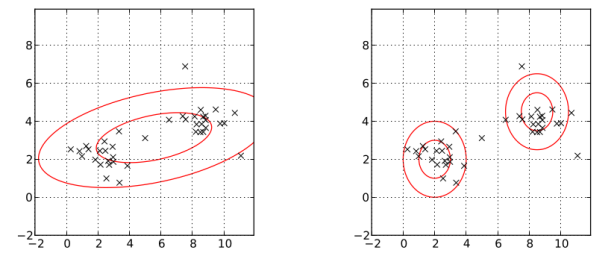
\includegraphics[width=\linewidth]{gaussian_moe.png}
  \caption{Left: Fit with one Gaussian distribution. Right: Fit with Gaussian
  mixture of 2 experts~\cite{mcgonagle_dobre_pilling}}
  \label{fig:gaussian_moe}
\end{figure}
%
This technique uses a gating network to divide the input space $x \in
\mathcal{X} \subset \mathbb{R}^{2m}$ into state partitions within which a single
expert is active.
%
The objective is to learn the expert models and the gating network that
best fit the dataset.
%

The expert models and the gating networks can take several forms. 
%
Gaussian experts and gating networks are commonly used in the MOE framework to
find a multi-modal probabilistic model from a small amount of
data~\cite{bishop2006pattern}.
%
However, as the observations from the dataset grow large, the Gaussian experts
impose large computational and memory overhead~\cite{harkonen2022mixtures}.
%
Moreover, Gaussian gating networks can only provide a quadratic parameterization
of the boundaries of the state partitions.
%
Hence, we leverage the universal approximation capabilities of neural networks
for both the experts and the gating network.
%


Let $F(x)$ denote a collection of $N_F$ expert models $F(x) = \{F_1(x),
\dots, F_{N_{F}}(x)\}$, whose parameters are given by the set
$\theta=\{\theta_1, \dots, \theta_{N_{F}} \}$.
%
% Henceforth, we assume that the number of state partitions is the same as the
% number of available expert controller.
%
The gating network $\mathbf{P}(x| \psi) := (P_1(x| \psi), \\ \dots, P_{N_F}(x|
\psi))$ is a collection of probabilities, where $P_i(x | \psi)$ denotes the
probability of state $x$ belonging to state partition $i, i \in \{1, \dots, N_F \}$. 
%
We parameterize the gating network with a neural network $\mathbf{P}(x| \psi) :
\mathcal{X} \rightarrow \mathbb{R}^{N_F}$ with parameters $\psi$, and the output
corresponds to the vector $[P_1(x| \psi), \dots, P_{N_F}(x| \psi)]$.
%
We use a \textsc{Softmax} activation function on the last layer to ensure that the
probabilities $P_i(x | \psi)$ over all state partitions $i$ sum to one.
%
The objective is to learn the decision parameters $(\psi, \theta)$ from observed
data.

We use a categorical probability distribution to sample a state partition based
on the outputs of the gating network as follows~\cite{harkonen2022mixtures} 
\begin{align}
  i | x, \psi \sim \text{Categorical}(\mathbf{P}(x| \psi)). 
  \label{eq:gating_categorical}
\end{align}
%
The prediction from the mixture of experts $F(x; \theta)$ is given by the linear
combination over the \it{responsibility} \normalfont of each state partition.
%
\begin{align*}
  I &= \underset{i}{\textrm{argmax}} \{ P_i(x | \psi) \}\\
  F(x; \theta) &= F_I(x; \theta_I)
\end{align*}
% A single controller is active in each state partition hence the prediction $F_o(x)$ is equivalent to 
% \begin{align*}
%   j &= \underset{i}{\textrm{argmax}} \{ P(c_i=i | x, \psi) \}\\
%   F_o(x) &= F_j(x)
% \end{align*}



There are several Bayesian inference techniques to learn the parameters of the
expert models and the gating network, one of which is \it{expectation
maximization} \normalfont (EM).
%
In this technique, we compose the expectation over the log likelihood
as~\cite{bishop2006pattern}   
\begin{equation}
  \mathbb{L}(\mathbb{D} | \theta, \psi) := \frac{1}{N} \sum_{j=1}^{N} \sum_{i=1}^{N_F} -\norm{F_i(x_j; \theta_i) - y_j}{}^2 P_i(x_j | \psi) 
  \label{eq:log_normal_likelihood}
\end{equation}
\noindent where $\mathbb{D} = \{(x_1, y_1), \dots, (x_N, y_N)\}$ is a collection
of $N$ training datasets, and $\norm{F_i(x_j; \theta_i) - y_j}{}$ is the error in the
prediction made by the expert $i$.
%
% We can expand this expression to 
% \begin{align}
%   \ln \{P(Y_x | \theta, \psi) \} = \sum_{j=1}^{N} \ln  \Biggl\{ \sum_{i=1}^{N_F} \mathcal{N}( \norm{F_i(x_j) - y_j}{}, s) P_i(x_j, \psi) \Biggr\}.
%   \label{eq:log_normal_likelihood}
% \end{align}
% %
% We can extract the relevant parts of~\eqref{eq:log_normal_likelihood} and define the
% final form of the likelihood function as
% \begin{align}
%   \mathbb{L}(Y_x | \theta, \psi) := \sum_{i=1}^{N_F} - \norm{F_i(x) - Y_x}{}^2 + \ln \Bigl\{ P(c_i=i | x, \psi) \Bigr\}.
%   \label{eq:likelihood_def}
% \end{align}
Notice that the likelihood measures how likely the current parameters $(\psi,
\theta)$ are to generate the sampled data $\mathbb{D}$. 
%
The goal is to maximize the likelihood and consequently minimize prediction
error.
%
The likelihood~\eqref{eq:log_normal_likelihood} is maximum when the parameter $\theta_i$
has the lowest prediction error and the highest probability of getting selected
by the gating network.
%
The standard EM approach evaluates~\eqref{eq:log_normal_likelihood} and uses
gradient-based techniques to iteratively update the parameters $(\psi, \theta)$.
%